\chapter{Design}
\label{chapter:design}

This chapter presents an in-depth discussion of the system's design, examining
the overall architecture, the rationale behind key design decisions, and the
unique aspects that distinguish this project.

\section{System Architecture Overview}

At a high level, the system comprises several loosely coupled components that
work together to enable remote gameplay on the Nintendo Wii console.
Figure~\ref{fig:expanded_overview} illustrates the primary components
and their interactions.

The primary subsystems include:
\begin{itemize}
	\item \textbf{Controller Input Relay}
	      A custom Python script acts as an intermediary, capturing input events
	      (such as accelerometer data, IR signals, and button presses) using the
	      \texttt{xwiimote} library\cite{xwiimote} and translating them into a binary
	      format. The script transmits these updates over UDP\cite{wikipediaUDP} to a Wiimote emulator running on the host machine.

	\item \textbf{Wii Remote Emulator:}
	      The emulator, derived from a fork\cite{jr_wiimote_emu} of the
	      \linebreak \texttt{WiimoteEmulator} project\cite{wiimote_emulator}, interprets the incoming
	      UDP packets and simulates the corresponding Wii Remote inputs, which are then
	      relayed to the Wii console via a Bluetooth connection. This project extends the
	      emulator's functionality to include streaming IR and accelerometer data over
	      UDP, which is essential for emulating the Wii Remote's motion controls based on
	      the remote player's inputs.

	\item \textbf{Audio and Video Streaming:}
	      An audiovisual streaming component enables remote gameplay by capturing
	      video and audio outputs from the Wii console. The system transmits these streams
	      to a client machine via the host machine using the Real-time Transport Protocol
	      (RTP)\cite{wikipediaRTP}.

	\item \textbf{Automation and Deployment:}
	      An automation script applies system configurations  -- such as loading
	      kernel modules and installation of dependencies  -- consistently across
	      devices.  The setup is tedious, error-prone, and not user-friendly without
	      automation. This problem compounds when considering the need to deploy the
	      system across multiple devices for users of varying technical expertise.
\end{itemize}

\section{Controller Input Relay}

\subsection{Design Rationale}
The relay is a custom Python script, leveraging Python’s rapid development capabilities and its extensive library support. The integration with the \texttt{xwiimote} library was particularly attractive because it allowed for the efficient capture of diverse input events (e.g., accelerometer readings, IR signals, and button presses). This design decision provided a robust platform that could quickly adapts when new input modalities or requirements emerge.

\subsection{Communication Strategy}
The relay utilises fixed-length binary packets that transmit over UDP to minimise communication latency and relay each sensor event in as close to real time as possible. The choice of UDP, despite its lack of error-checking compared to TCP\cite{wikipediaTCP}, was deliberate: it reduces overhead and is better suited for applications where timely data delivery is more critical than guaranteed packet delivery. All of the I/O operations in the relay are non-blocking, further enhancing responsiveness and ensuring that the system remains highly interactive.

\subsection{Modularity and Extensibility}
Modularity was a guiding principle in the relay’s design. By mapping all input types to a unified binary format, the system remains adaptable. New sensors, like Wii MotionPlus\cite{wikipediaMotionPlus} or alternate controllers, like nunchucks, can integrate without significant changes to the core architecture. This design supports future enhancements while maintaining a clear separation between data acquisition, processing, and transmission.

\section{Wiimote Emulator}

\subsection{Leveraging Established Codebase}
Instead of developing a Wii Remote emulator from scratch, the project builds upon the \texttt{WiimoteEmulator} project. Building a new Wii Remote emulator would have been too time-consuming and risked introducing bugs. One benefit of building an emulator from scratch would be the ability to minimise the latency between the emulator and the Wii console -- something that the \texttt{WiimoteEmulator} project didn't focus on. However, the latency introduced by the emulator doesn't make the games unplayable, as shown in the \nameref{sec:playability-analysis} section. Adapting an existing project allowed for a focus on design improvements rather than foundational re-implementation.

\subsection{Enhanced Input Simulation}
Extensions to the emulator support streaming IR and accelerometer data over UDP. This feature enables the remote player’s inputs to be accurately reflected in the Wii console’s gameplay. The original \texttt{WiimoteEmulator} project is able to emulate IR and accelerometer data but only through a mouse and keyboard interface. In addition, the original project calculates all the IR and accelerometer data in small movements, i.e. there is no way to quickly snap from one end of the screen to the other. Thus, the improvements to the \texttt{WiimoteEmulator} project centre around fixing these shortcomings.

\section{Audio and Video Streaming}

\subsection{Protocol Selection}
Adopting the Real-time Transport Protocol (RTP) leverages its framework for live
media streaming. RTP’s design supports low-latency transmission, which is
essential for achieving the lowest latency possible. The use of other protocols, like
UDP, was considered but ultimately rejected due to the lack of built-in support for
audio and video streaming. It is not the use of RTP alone that reduces latency but the
specific configurations that the protocol allows for which UDP does not.

\subsection{Use of FFmpeg and FFplay}
The system relies on FFmpeg\cite{wikipediaFFmpeg} and FFplay\cite{ffplay} for capturing and streaming audiovisual data. FFmpeg’s extensive codec support and FFplay’s real-time playback capabilities make them well-suited for this application. The design leverages these tools to ensure seamless audiovisual streaming, with FFplay providing a low-latency display of the Wii’s output on the client machine. Notably, this requires remote users to use FFplay, or similar tools that integrate with FFmpeg, to view the game stream. This restricts users to a possibly unfamiliar interface, but ensures a consistent experience across all clients.

\section{Automation and Deployment}

\subsection{Centralised Configuration Management}
A comprehensive setup script manages configuration tasks -- such as loading essential kernel modules, updating Bluetooth settings, and installing necessary libraries. Centralising these tasks into an automated process reduces the risk of inconsistencies and ensures that every deployment starts from a known baseline.

\subsection{Accessibility and Usability}
The automation script priorities user-friendliness and accessibility. By abstracting complex setup procedures into a single command, the script lowers the barrier to entry for users who may lack technical expertise. This design choice aligns with the project’s goal of providing an accessible and intuitive remote gaming experience meant for a broad audience.

\subsection{Scalability and Future-Proofing}
A key design decision was to ensure that the deployment process could scale with the system. The automation script is easy to extend and can incorporate new configuration steps when new features or requirements arise. This foresight in design allows the system to evolve without necessitating a complete overhaul of the deployment process, thereby supporting long-term scalability and maintainability.

% \section{Component-Level Design and Data Flow}

% The system’s architecture emphasises clear data flow and modularity. Figure~\ref{fig:expanded_overview} illustrates the primary components and their interactions.

% % \begin{figure}[h]
% % 	\centering
% % 	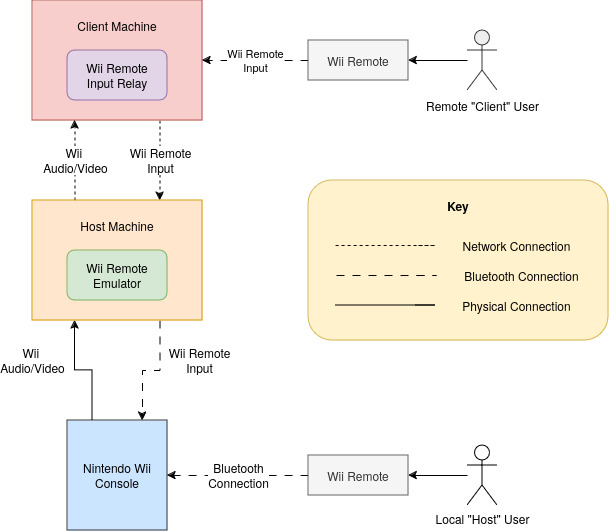
\includegraphics[width=0.9\textwidth]{advanced_intro.jpg}
% % 	\caption{System Architecture and Data Flow}
% % 	\label{fig:architecture}
% % \end{figure}

% At the core of the design is the input relay mechanism, which operates as follows:

% \begin{enumerate}
% 	\item \textbf{Input Capture:}
% 	      The Wii Remote’s events are captured using the \texttt{xwiimote} library. Both analog (accelerometer, IR) and digital (button press) events are monitored continuously.

% 	\item \textbf{Event Processing:}
% 	      In the Python script, events are handled in a non-blocking manner using \texttt{select.poll()}. The script processes each event by normalising sensor data and mapping it into the expected range. For example, IR data is normalised to a [0,1] scale and then converted to a resolution that matches the Wii’s requirements, while accelerometer data is similarly scaled.

% 	\item \textbf{Packet Formation and Transmission:}
% 	      Processed events are packaged into binary data packets. The design utilises fixed-length packets with a dedicated header byte to distinguish between different types of events (e.g., \texttt{0x01} for IR and \texttt{0x02} for accelerometer data). These packets are transmitted over UDP to the emulator, which interprets them to simulate the corresponding inputs.

% 	\item \textbf{Emulation and Output:}
% 	      The emulator on the host Raspberry Pi receives the UDP packets and integrates the data into its internal state. The emulation layer uses transformation routines to convert the incoming data into the simulated state of the Wii Remote, including generating IR positions and accelerometer readings.
% \end{enumerate}

\section{Novel Design Features}

\subsection{Responsive Motion Control Emulation}
The system’s motion control emulation is a novel feature that enables remote players to interact with the game in real-time. By streaming IR and accelerometer data over UDP, the system accurately reflects the remote player’s inputs on the Wii console. Allowing a remote user to control the game as if they were physically present is a unique design feature that enhances the system’s immersive qualities.

\subsection{Local Play Game Features}
Other third party projects, like \texttt{wiimmfi}\cite{wiimmfi}, have focused on replicating the functionality of the Wii’s original online services. However, many Nintendo Wii games have specific gameplay features that require local multiplayer or never supported online play -- such as Wii Sports. This project’s focus on enabling local multiplayer experiences over IP is a unique design feature that caters to a broader range of games and plugs a gap in the existing ecosystem.

\subsection{Automated Environment Configuration}
Automates device setup by configuring kernel modules, adjusting Bluetooth configuration files, and installing necessary dependencies through a comprehensive script. This minimises configuration errors and drastically reduces setup time, ensuring that all devices operate from a consistent baseline. This design feature simplifies the deployment process, making the system accessible to users with varying technical expertise. The focus on accessibility and usability is novel in the context of remote gaming systems, where complex configurations can be a significant barrier to entry\cite{dirkBarrierToEntry}.

%% \section{Design Trade-offs and Considerations}

%% Throughout the design process, several trade-offs were considered:

%% \begin{itemize}
%%     \item \textbf{Latency vs. Quality:}
%%           The dual requirements of maintaining low latency and high-quality audiovisual output necessitated careful balancing. The use of RTP with specific broadcast and play parameters emerged as the optimal solution, though some latency issues remain, particularly in the synchronisation between the input relay and the video stream.

%%     \item \textbf{Complexity vs. Modularity:}
%%           While modular design enhances maintainability and scalability, it also introduces complexity in terms of interfacing between different subsystems.

%%     \item \textbf{Performance vs. Flexibility:}
%%           The decision to implement performance-critical components in C ensures fast processing of sensor data but at the cost of reduced flexibility compared to a pure Python solution. The hybrid approach adopted here strikes a balance by enabling rapid development in Python for higher-level functions while reserving C for tasks where performance is paramount.
%% \end{itemize}
